\section{E4: Preis einer Adaption}
\label{app:report_e4}
\subsection*{Setup}
\begin{itemize}
\item \textbf{Lauf:} e4\_\allowbreak{}004
\item \textbf{Stichtage:} SF6: 02.12.2016, SF7: 13.01.2017, SF8: 20.02.2017
\item \textbf{Szenarien:} peak, level, dazu der Kontrolllauf
\item \textbf{Systeme:} SYS3 mit Adaption
\item \textbf{Sprachmodell:} ministral-3:8b, Prompt v30, ohne Kalender (CTX0)
\item \textbf{Einbautage:} je Lauf ein Einbau an Tag 3, 10, 18, 26, 35, 43, 51
\item \textbf{Starthistorie:} 7 und 60 Tage
\item \textbf{Auswertung:} 56 Tage ab dem Start in Wochen zu 7 Tagen, je Stichtag dieselben Kalendertage für beide Starthistorien
\item \textbf{Prognosemodelle:} C3\_\allowbreak{}60 täglich nachtrainiert, C1 statisch, nur auf der Starthistorie trainiert
\item \textbf{Commit:} abb4823
\end{itemize}

\subsection*{Kriterien der Teilfrage 4}
\begin{tablang}{W{1.49} W{0.58} W{1.53} W{0.40}}{Kriterium & Ziel & Ergebnis & erfüllt}
Tagesfehler bei 7 Tagen belastbar höher & 0 Wochen & 0 von 8 & ja \\
zusätzliches Zurücksetzen & 0 Läufe & 13 von 45 & nein \\
Erkennungsrate, 7 bezogen auf 60 Tage & $\geq$ 90 \% & 14 von 27 (52 \%) & nein \\
Tagesfehler, C3\_\allowbreak{}60 minus C1, 7 Tage & < 0, belastbar & \textminus{}676,5 W, 2 Standardfehler 177,9 W, belastbar & ja \\
\end{tablang}

\subsection*{Kennzahlen über alle Starttermine, Starthistorie 7 gegen 60 Tage}
\begin{tablang}{W{1.94} W{0.55} W{0.51}}{Kennzahl & 7 Tage & 60 Tage}
Tagesfehler C3\_\allowbreak{}60 [W] & 92,8 & 95,5 \\
Tagesfehler C3\_\allowbreak{}60 minus C1 [W] & \textminus{}676,5 & \textminus{}121,1 \\
Erkannte Einzelanomalien (erwartete Klasse am Tag nach dem Einbau) & 18 von 42 & 27 von 42 \\
Tage im Kontrolllauf, an denen nur bei 7 Tagen gemeldet wird & 7 von 168 & - \\
Tage im Kontrolllauf, an denen nur bei 60 Tagen gemeldet wird & 10 von 168 & - \\
Läufe mit Zurücksetzen nur bei 7 Tagen & 13 von 45 & - \\
\end{tablang}

\begin{landscape}
\subsection*{Starthistorie 7 gegen 60 Tage je Woche nach dem Start}
\begin{tablang}[\footnotesize\setlength{\tabcolsep}{3pt}]{W{0.64} W{1.28} W{1.12} V{0.88} V{0.88} W{0.88} W{0.88} V{1.44}}{Woche & Differenz Tagesfehler [W] & belastbar & Meldung nur bei 7 & Meldung nur bei 60 & erkannt bei 7 & erkannt bei 60 & Zurücksetzen nur bei 7}
1 & \textminus{}2,4 & nein & 1 & 2 & 1 von 6 & 5 von 6 & 0 \\
2 & \textminus{}1,6 & nein & 0 & 1 & 2 von 6 & 6 von 6 & 0 \\
3 & \textminus{}5,4 & nein & 0 & 3 & 1 von 6 & 4 von 6 & 0 \\
4 & \textminus{}7,4 & nein & 0 & 0 & 4 von 6 & 4 von 6 & 0 \\
5 & 1,1 & nein & 0 & 2 & - & - & 0 \\
6 & \textminus{}5,5 & nein & 4 & 1 & 4 von 6 & 2 von 6 & 13 \\
7 & 0,6 & nein & 2 & 0 & 4 von 6 & 4 von 6 & 0 \\
8 & \textminus{}0,8 & nein & 0 & 1 & 2 von 6 & 2 von 6 & 0 \\
gesamt & \textminus{}2,7 & nein & 7 & 10 & 18 von 42 & 27 von 42 & 13 \\
\end{tablang}
\end{landscape}

\subsection*{Einschwingwoche: erste Woche, ab der es keine Abweichung mehr gibt}
\begin{tablang}{W{0.67} W{1.33}}{Größe & ab Woche}
Prognose & 1 \\
Meldungen & nicht eingeschwungen \\
Erkennung & nicht eingeschwungen \\
\end{tablang}

\subsection*{Hinweise}
\begin{itemize}
\item Tag 0 = erster prognostizierter Tag, an ihm wird der letzte Tag der Starthistorie eingeordnet. Ein Einbau an Tag k wird an Tag k + 1 eingeordnet
\item Als Meldung zählen die Klassen peak, new\_\allowbreak{}pattern, measurement\_\allowbreak{}error. Abweichende Meldungen werden im Kontrolllauf am selben Tag verglichen. Es sind echte Daten, eine Meldung nur bei 7 Tagen kann also berechtigt sein
\item Erkennungsrate: von den Einzelanomalien, die bei 60 Tagen am Tag nach dem Einbau mit der erwarteten Klasse eingeordnet werden, der Anteil, den auch 7 Tage so einordnen, über alle Tage
\item zusätzliches Zurücksetzen: Läufe, in denen bei 7 Tagen zurückgesetzt wird und bei 60 Tagen am selben Tag nicht, je Lauf einmal gezählt
\item Einschwingwoche: Prognose nach der 2-Standardfehler-Regel, Meldungen nach jedem abweichenden Tag, Erkennung nach jeder Einzelanomalie, die nur die lange Starthistorie erkennt. Die Erkennung ist nur bis zur letzten Woche mit Einbau belegt
\item belastbar: Betrag der Differenz größer als 2 Standardfehler der gepaarten Differenzen, grobe Faustregel
\item Tagesfehler je Tag seit dem Start im Plot: Mittel über die Starttermine, über 7 Tage geglättet
\end{itemize}
\begin{center}
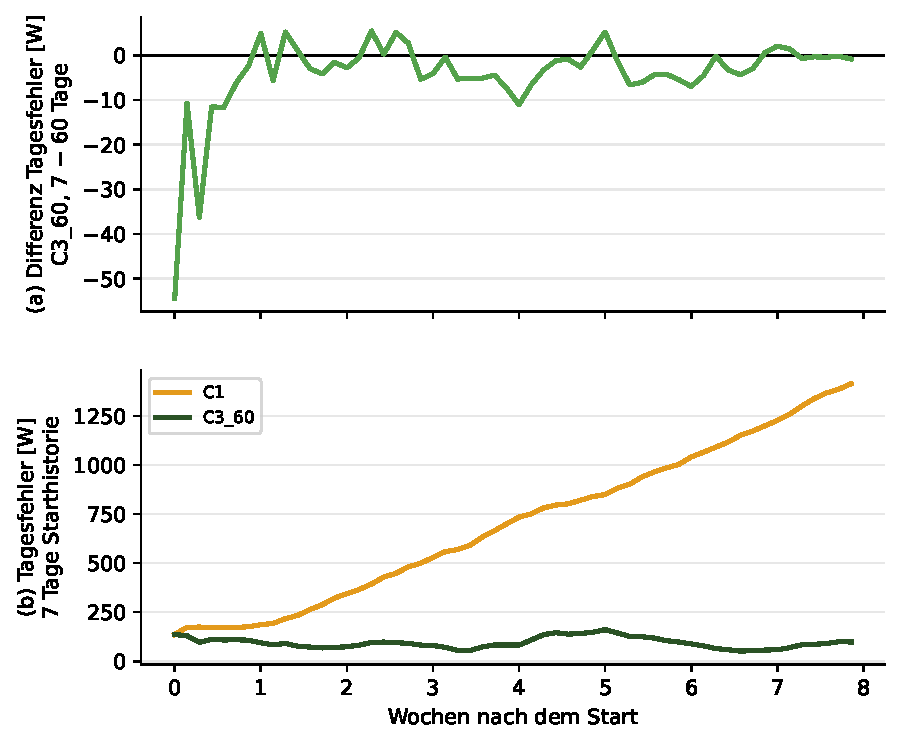
\includegraphics[width=\linewidth]{e4_forecast.pdf}
\end{center}
\begin{center}
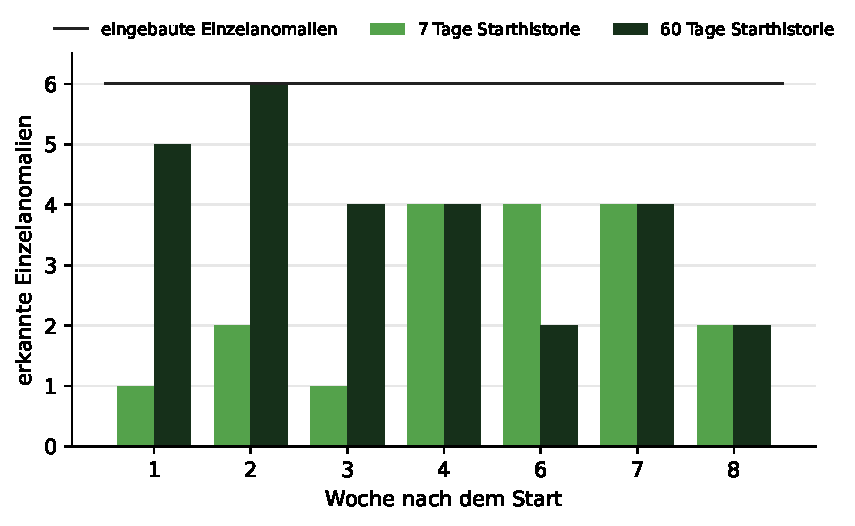
\includegraphics[width=\linewidth]{e4_detection.pdf}
\end{center}

\subsection*{Weitere Tabellen}

\subsubsection*{Tagesfehler C3\_\allowbreak{}60 minus C1 je Woche nach dem Start [W], negativ = C3\_\allowbreak{}60 besser}
\begin{tablang}{V{0.96} V{1.08} V{0.96}}{Woche & 7 Tage & 60 Tage}
1 & \textminus{}68,4 & \textminus{}15,0 \\
2 & \textminus{}251,8 & \textminus{}56,1 \\
3 & \textminus{}417,1 & \textminus{}86,8 \\
4 & \textminus{}617,7 & \textminus{}102,2 \\
5 & \textminus{}692,0 & \textminus{}157,4 \\
6 & \textminus{}905,5 & \textminus{}159,6 \\
7 & \textminus{}1143,3 & \textminus{}228,3 \\
8 & \textminus{}1316,1 & \textminus{}163,2 \\
\end{tablang}

\subsubsection*{Zusätzliches Zurücksetzen nur bei 7 Tagen, je Lauf}
\begin{tablang}{W{1.14} W{1.00} V{1.00} V{1.29} W{0.57}}{Starttermin & Szenario & Einbautag & Zurücksetzen am Tag & Skala}
SF7 & peak & 10 & 35 & weekly \\
SF7 & peak & 18 & 35 & weekly \\
SF7 & peak & 26 & 35 & weekly \\
SF7 & level & 18 & 36 & weekly \\
SF7 & level & 26 & 36 & weekly \\
SF7 & Kontrolllauf & - & 37 & weekly \\
SF7 & peak & 35 & 37 & weekly \\
SF7 & peak & 43 & 37 & weekly \\
SF7 & peak & 51 & 37 & weekly \\
SF7 & level & 3 & 37 & weekly \\
SF7 & level & 35 & 37 & weekly \\
SF7 & level & 43 & 37 & weekly \\
SF7 & level & 51 & 37 & weekly \\
\end{tablang}

\begin{landscape}
\subsubsection*{Eingebaute Einzelanomalien: $\checkmark$ = erwartete Klasse am Tag nach dem Einbau, – = nicht}
\begin{tablang}[\footnotesize\setlength{\tabcolsep}{3pt}]{W{1.41} V{1.65} W{0.82} W{0.82} W{0.82} W{0.82} W{0.82} W{0.82}}{Szenario & Einbautag & SF6, 7 Tage & SF6, 60 Tage & SF7, 7 Tage & SF7, 60 Tage & SF8, 7 Tage & SF8, 60 Tage}
level & 3 & – & $\checkmark$ & – & $\checkmark$ & – & $\checkmark$ \\
level & 10 & – & $\checkmark$ & – & $\checkmark$ & – & $\checkmark$ \\
level & 18 & – & – & – & $\checkmark$ & – & $\checkmark$ \\
level & 26 & – & – & $\checkmark$ & $\checkmark$ & $\checkmark$ & $\checkmark$ \\
level & 35 & $\checkmark$ & – & – & – & $\checkmark$ & $\checkmark$ \\
level & 43 & $\checkmark$ & – & – & – & $\checkmark$ & $\checkmark$ \\
level & 51 & $\checkmark$ & – & – & – & – & – \\
peak & 3 & – & $\checkmark$ & $\checkmark$ & $\checkmark$ & – & – \\
peak & 10 & – & $\checkmark$ & $\checkmark$ & $\checkmark$ & $\checkmark$ & $\checkmark$ \\
peak & 18 & – & – & $\checkmark$ & $\checkmark$ & – & $\checkmark$ \\
peak & 26 & – & – & $\checkmark$ & $\checkmark$ & $\checkmark$ & $\checkmark$ \\
peak & 35 & $\checkmark$ & – & – & – & $\checkmark$ & $\checkmark$ \\
peak & 43 & $\checkmark$ & $\checkmark$ & – & $\checkmark$ & $\checkmark$ & $\checkmark$ \\
peak & 51 & $\checkmark$ & $\checkmark$ & – & $\checkmark$ & – & – \\
\end{tablang}
\end{landscape}
